In Chapter \ref{ch:languages} we showed an implementation in Metacasanova of Casanova, a domain-specific language for game development and we discussed the reason of the poor performance of that implementation. In Chapter \ref{ch:functors} we extended Metacasanova with functors and modules to allow to embed the type system of an embedded  language \footnote{See the introduction of Chapter \ref{ch:functors} for a definition of this term} in the meta-compiler to overcome the problem of dynamic lookups at runtime. We then showed an implementation of records with modules and functors that significantly improved the performance of memory accesses, as shown in Section \ref{sec:ch_functors_evaluation}. In this chapter we show how this language extension can be used to improve the performance of the implementation in Metacasanova of the domain-specific language for game development Casanova. In what follows we start by describing how entities are updated in Casanova to make their dynamics evolve with respect to time. We then proceed to discuss how functors can be used to describe the semantics of entity updates in Casanova, and we further refine it to support the semantics of interruption of Casanova rules. We conclude with an evaluation about the performance gain achieved by using this implementation over the previous one presented in Chapter \ref{ch:languages}.

\section{Casanova entity update}
\label{subsec:ch_networking_casanova_update}
In Section \ref{subsec:ch_mcnv_languages_casanova_semantics} we described the memory representation of a Casanova entity in Metacasanova and how the rules of an entity are updated. What was skipped for brevity was a description of how the system behind Casanova updates the entities of a Casanova program. As briefly described in Section \ref{sec:ch_mcnv_languages_casanova_language}, the structure of a program in Casanova is a tree, whose root is a special entity called \textit{World}. The world entity can contain fields that are instances of other entities as well, thus creating an additional level in the program tree. This is, of course, allowed also for regular entities, thus the height of the tree is arbitrary. Each entity might contain a set of rules that describe its dynamic behaviour with respect to time, thus they are updated by considering the time difference between the current and the previous update (\textit{frames}). Updating a rule is enforced by traversing the entity tree, thus when the field of an entity is an entity itself, the system will first update the entity instance contained in the field and then update the current entity. Casanova also natively supports lists and tuples as valid data types, and this requires to handle their update as well: a tuple or a list might themselves contain instances of entities that must be updated accordingly. In the case of a list of entities, we must run the update on each element, while in the case of a tuple we must examine each element and check whether it requires an update or not. This process is called \textit{update traversal} and might become very complex, as lists and tuples can be combined together in infinite many ways, thus the process recursively calls the proper update depending on the type of the field.

For instance, let us consider a simulation consisting of an arbitrary number of physical bodies, in the fashion of what was used in Section \ref{subsec:ch_functors_casanova_example}. The world entity will contain a list of physical bodies that are updated during the simulation. The Casanova code that described such a simulation is the following:

\begin{lstlisting}
worldEntity World {
	PhysicalBodies : [PhysicalBody]
}

entity PhysicalBody {
	Position				: Tuple<float,float>
	Velocity				: Tuple<float,float>
	Acceleration		: Tuple<float,float>
	
	rule Position = Position + Velocity * dt
	rule Velocity = Velocity + Acceleration * dt
}
\end{lstlisting}

\noindent
In this simulation, the update starts from \texttt{World}. This entity contains only one field, which is a list of physical bodies. Since \texttt{PhysicalBody} is an entity, the update must be run individually for each element of the list. The world contains no rules, thus after updating its only field we complete its update. At this point the update of each of the physical body examines each fields. All fields are represented as a point in a 2D space with a tuple containing two floating-point values. The update will examine each value of the tuple and find that they do not require any update (again because the only language abstractions that exhibit dynamic behaviours are entities). The update will then move on to run the rules that will update the content of \texttt{Position} and \texttt{Velocity}. The update process is sketched in Figure \ref{fig:ch_networking_simulation_update} and can thus be seen as a process that consists of the following steps:

\begin{enumerate}[noitemsep]
	\item An \textit{entity update} that traverses all the fields and rules of the entity and calls the appropriate updater.
	\item A \textit{field update} that updates (or not) the field depending on its type. The fields that will be updated have type \texttt{List}, \texttt{Tuple}, or \texttt{Entity}.
\end{enumerate}

\begin{figure}
	\centering
	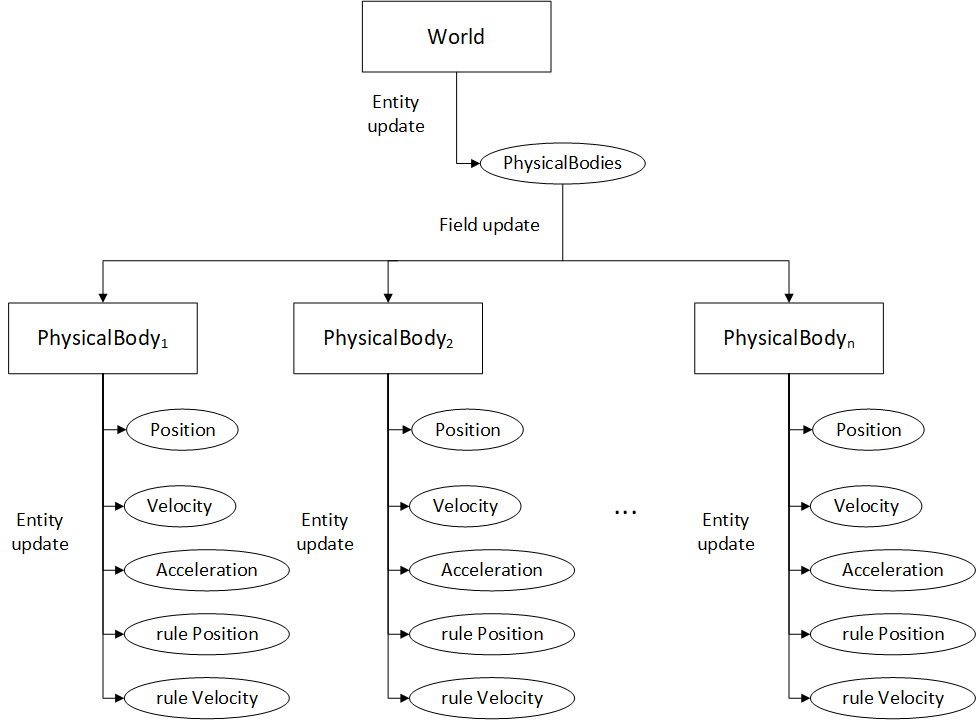
\includegraphics[width=\textwidth]{Figures/chapter_networking/update_traversal}
	\caption{Entity update for the simulation of physical bodies}
	\label{fig:ch_networking_simulation_update}
\end{figure}

\section{Update in Metacasanova}
\label{subsec:ch_networking_update_metacasanova}
The update mechanism described in Section \ref{subsec:ch_networking_casanova_update} can of course be integrated in the implementation of Casanova described in Chapter \ref{ch:languages}. In order to do so, we should dynamically look into the dictionary representing the entity fields at each update, extract the field and perform an update according to the following cases:

\begin{itemize}[noitemsep]
	\item If the field is a list, then we must examine each element and choose for each one whether it needs to be updated or not. This is done by recursively applying these cases (being a dynamic check we have to perform this check for each element).
	\item If the field is a tuple, then we behave as above.
	\item If the field is an entity, then we must run an update on it.
	\item In all the other cases the field is not updated.
\end{itemize}

\noindent
The cases above are translated into four rules in Metacasanova. The first three will use pattern-matching to decide whether the examined field is a list, a tuple, or an entity. The fourth one is a default rule that simply returns the field as it is. Moreover, each entity should store a list of rules that are updated as well, where all the get and set operations require dynamic lookups in the symbol table of the entity.

Repeating the traversal of the entity tree at each update at runtime is unnecessary since

\begin{itemize}[noitemsep]
	\item The structure of a Casanova entity cannot change at runtime. Its fields and field types will always remain the same.
	\item The fields affected by an entity rule and the rules of an entity do not change during the program execution.
\end{itemize}

\noindent
This means that, by exploiting modules and functors, we are able to specify the structure of the update at compile time and generate directly the function that performs the update at runtime, in the same fashion as what has been done for the record setter and getter. In the following sections we will describe extensively the implementation of the update using modules and functors in Metacasanova that generates at compile time the functions necessary to perform the update of a Casanova program. Note that we will refer to the implementation of records given in Section \ref{sec:ch_functors_record_implementation}.

\section{Updater Modules}
\label{subsec:ch_networking_updater_modules}
As explained above, Casanova needs to recursively update fields that are lists, tuples, or entity instances. For this purpose, we define a module that represents an \textit{updatable element} in the Casanova language. The module constructor takes as only argument the type of the element to update. This module contains a function \texttt{update} that is able to update a value of this particular type and uses an additional parameter \texttt{dt} that contains the time difference between the current and the previous update. The function returns the updated value of the element. It also contains an utility functor to return the type of the element.
 
\begin{lstlisting}
Module "ElementUpdater" => (elementType : *) : ElementUpdater {
	Functor "GetType" : *
	Func "update" -> elementType -> float : elementType
}
\end{lstlisting}

\noindent
The updater for a field is a module constructed by providing the record of the fields, its name as a string, and contains: (\textit{i}) an utility functor that returns the record used in the field updater, and (\textit{ii}) an update function that takes as input an instance of the record, \texttt{dt}, and returns the updated value of the field. We also define an external utility functor \texttt{GetFieldType} that can retrieve the type of a record field given the record it belongs to and its name. The rule for the functor calls the field getter and its \texttt{GetType} functor to retrieve the type of the field. This functor is used by the module constructor to correctly generate the return type of the \texttt{update} function.

\begin{lstlisting}
Functor "GetFieldType" => Record => string : *

GetField r name => getter
getter.GetType => type
---------------------------
GetFieldType r name => type

Module "FieldUpdater" => (r : Record) => (name : string) : FieldUpdater {
  Functor "GetRecord" : Record
  Func "update" -> r.RecordType -> float : (GetFieldType r name)
}
\end{lstlisting}

\noindent
Finally, the updater for a record is a module constructed by providing the record itself and contains: (\textit{i}) an utility functor that returns the type of the record, and (\textit{ii}) a function \texttt{update} that takes the instance of the record, \texttt{dt}, and returns an updated instance of the record.

\begin{lstlisting}
Module "RecordUpdater" => (r : Record) : RecordUpdater {
  Functor "RecordType" : *
  Func "update" -> r.RecordType -> float : r.RecordType
}
\end{lstlisting}

\section{Updatable elements}
\label{subsec:ch_networking_updatable_elements}
As explained above, the elements for which the update is needed can be lists, tuples, or entity instances. For this reason we have to create separately three different instances of the module \texttt{ElementUpdater} each one dedicated to updating one of those updatable elements. The first updatable element that we consider is an \textit{entity instance}. The module to update such updatable element uses a \texttt{RecordUpdater} to define how the entity instance should be updated. Updating a field containing an entity instance requires the application of the specific record updater for that entity, which in turn returns the updated instance of the entity itself. Thus the declaration for the functor that constructs the proper instance of the module for the entity updater is the following:

\begin{lstlisting}
Functor "UpdateEntity" => RecordUpdater : ElementUpdater
\end{lstlisting}

\noindent
The rule for this functor extracts in its premise the type of the record by calling the utility functor \texttt{RecordType} in the record updater passed as parameter to \texttt{UpdateEntity}. The \texttt{update} function uses the record updater to recursively update the entity instance in its premise and then returns the result of this update.

\begin{lstlisting}
recordUpdater.RecordType => recordType
--------------------------
UpdateEntity recordUpdater => ElementUpdater recordType {

	----------------------
	GetType => recordType
 
  recordUpdater.update entity dt -> entity'
  ------------------------------
  update entity dt -> entity'
}
\end{lstlisting}

\noindent
The second updatable element is the list. An updater for a list must take the updater for its elements. Since a list contains elements of the same type, only one updater is required to instantiate its updater module. The functor \texttt{UpdateList} used to generate this module takes one argument which is an \texttt{ElementUpdater}. This is done because the elements of a list could be themselves other lists, entities, or tuples, so we must be able to use their updaters as arguments for this function. The declaration for this functor is thus:

\begin{lstlisting}
Functor "UpdateList" => ElementUpdater : ElementUpdater
\end{lstlisting}

\noindent
The rule for \texttt{UpdateList} extracts in its premise the type of the elements of the list by calling the functor \texttt{GetType} in the element updater provided as input. It then instantiates an \texttt{ElementUpdater} with the type \texttt{List} using as argument for the generic type the type of the element extracted in its premise. The \texttt{update} function for the list is recursive: its base case is the empty list, for which it simply returns an empty list. For a non-empty list the rule for this function uses the element updater in its premise to update the head of the list and then recursively calls the \texttt{update} of the list on the tail to update the remaining part.

\begin{lstlisting}
updater.GetType => elementType
---------------------------------
UpdateList updater => ElementUpdater List[elementType] {

  -----------------
  GetType => List[elementType]

  --------------------
  update nil dt -> nil

  updater.update x dt -> x'
  update xs dt -> xs'
  -------------------
  update (x :: xs) dt -> (x' :: xs')
}
\end{lstlisting}

\noindent
The updater for tuples is built by defining a functor that takes as input two element updaters, one for the current element of the tuple, and one for the second one. Note that it is possible to recursively provide a tuple updater as a second updater to support the update of tuples containing more than two elements. For example, the updater for \texttt{Tuple[PhysicalBody,Tuple[PhysicalBody,PhysicalBody]]} would require the passing of an entity updater and recursively a tuple updater. The declaration of this fuctor is thus:

\begin{lstlisting}
Functor "UpdateTuple" => ElementUpdater => ElementUpdater : ElementUpdater
\end{lstlisting}

\noindent
The rule for \texttt{UpdateTuple} uses in its premises \texttt{GetType} from the first updater and the second updater to obtain the types of the first and second element of the tuple. It then instantiates \texttt{ElementUpdater} with the tuple type called with the type of the first and second element as arguments for the generics. The \texttt{update} function runs the \texttt{update} of the first updater on the first element of the tuple and the second updater on the second element.

\begin{lstlisting}
updater.GetType => firstType
nextUpdater.GetType => nextType
---------------------------------------------
UpdateTuple updater nextUpdater => ElementUpdater Tuple[firstType,nextType] {

  -------------------
  GetType => Tuple[firstType,nextType]

  updater.update x dt -> x'
  nextUpdater.update x' dt -> xs'
  ----------------------
  update (x,xs) dt -> (x',xs')
}
\end{lstlisting}

Finally, we need a \texttt{ZeroUpdate} that is required for fields whose values do not change with respect to time, namely all those that do not fall in the three categories above. The functor \texttt{ZeroUpdate} takes as input any type and builds an \texttt{ElementUpdater} with that type. The rule for \texttt{update} simply returns the value of the field as it is.

\begin{lstlisting}
Functor "ZeroUpdate" => * : ElementUpdater

-----------------------
ZeroUpdate type => ElementUpdater type {

  ----------------
  GetType => type

  ----------------
  update v dt -> v
}
\end{lstlisting}

\section{Updatable Fields and Records}
The field updater is instantiated by a functor that takes as input an element updater, a record containing the field, and the name of the field to update. Its declaration is the following:

\begin{lstlisting}
Functor "UpdateField" => ElementUpdater => Record => string : FieldUpdater
\end{lstlisting} 

\noindent
The rule for the \texttt{update} function creates in its premises a field getter through the record and the field name passed as input. It then call the function \texttt{get} of the getter with the record instance taken as input to get the value of the field. It then uses the \texttt{update} function from the element updater taken as input from the functor to update the field.

\begin{lstlisting}
----------------------------------------
UpdateField elementUpdater r name => FieldUpdater r name {

  ---------------
  GetRecord => r

  GetField r name => getter
  getter.get rec -> field
  elementUpdater.update field dt -> field' 
  -----------------------------
  update rec dt -> field'
}
\end{lstlisting}

\noindent
The record updater is built by a functor \texttt{Update} that takes as input a field updater, a record updater to update the next part of the record, and returns an instance of the \texttt{RecordUpdater} module. The rule that evaluates the functor extracts the record from the field updater in its premise and passes it to the module constructor for the record updater. The rule for \texttt{update} generates a setter for the field by using the record and the field name. It then calls the field updater passing the record instance and \texttt{dt} as input. This premise will return the updated value for the field. The following premise uses the \texttt{set} function from the previously generated setter to update the record with the new value of the field. After this step it calls the \texttt{update} function of the record updater passed as function argument, which is recursively able to update the remaining part of the record. The result of this update is then returned as final result. Both the functor declaration and the rule for it are provided below

\begin{lstlisting}
Functor "Update" => FieldUpdater => RecordUpdater : RecordUpdater

fieldUpdater.GetRecord => r
---------------------------
Update fieldUpdater nextUpdater => RecordUpdater r {

  r.RecordType => recordType
  ------------------------
  RecordType => recordType

  SetField r name => setter
  fieldUpdater.update rec dt -> v
  setter.set rec v -> rec'
  nextUpdater.update rec' dt -> updatedRecord
  ----------------------------
  update rec dt -> updatedRecord
}
\end{lstlisting}

\noindent
Note that it is possible to provide different field updaters for the same field, as it is possible that, besides the standard Casanova traversal, one wants to define a custom way of updating the field through a Casanova rule.

In order to stop this otherwise infinite recursive process, we must also generate a record updater that simply returns the record as it is. We build such updater through the functor \texttt{NoUpdate}. This functor takes as input a record and instantiates its updater with it. The updater contains a rule for the \texttt{update} function that simply returns the record as it is. The implementation for this updater is provided below:

\begin{lstlisting}
Functor "NoUpdate" => Record : RecordUpdater

---------------------
NoUpdate r => RecordUpdater r {

  r.RecordType => recordType
  ----------------------
  RecordType => recordType
  
  ----------------
  update r dt -> r
}
\end{lstlisting}

\noindent
Finally, rules can be implemented as a field updater that is instantiated by a functor taking as input the record and the field name. The \texttt{update} function will contain the specific code that the rule will perform. In the following section we will provide the implementation of the physical body simulation and show how to use functors to generate the field updater for rules.

\section{Physical Body Simulation with Functors}
\label{subsec:ch_networking_simulation}
In this section we present the implementation with functors of the simulation in Casanova presented in Section \ref{subsec:ch_networking_casanova_update}. The simulation consists of a set of bodies that moves according to their physical properties. As previously done in Section \ref{sec:ch_functors_record_implementation}, we create a functor that builds the record module instance for the physical body:

\begin{lstlisting}
Functor "PhysicalBodyType" : Record

RecordField "Acceleration" Tuple[float,float] EmptyRecord => acceleration
RecordField "Velocity" Tuple[float,float] acceleration => velocity
RecordField "Position" Tuple[float,float] velocity => body
---------------------------
PhysicalBodyType => body
\end{lstlisting}

\noindent
At this point, we define the updaters for the physical body fields. Its fields consist of a tuple with two floating point values. Since floating-point values do not require to be updated in Casanova, we create an updater for the floating-point numbers by using the \texttt{ZeroUpdate} functor that instantiates \texttt{ElementUpdater} with an \texttt{update} function that simply returns the input value.

\begin{lstlisting}
Functor "FloatUpdater" : ElementUpdater

ZeroUpdate float => zero
--------------------------
FloatUpdater => zero
\end{lstlisting}

\noindent
\texttt{ZeroUpdate} calls \texttt{ElementUpdater} with \texttt{elementType := float}. The instance of this module will then contain the following functor rule and function declaration\footnote{Note that the evaluation rules in a functor are always the same for each instance of a module, so from now on we omit them for brevity}.

\begin{lstlisting}
Func "update" -> float -> float : float

-----------------
GetType => float
\end{lstlisting}

\noindent
At this point we can define the element updater for the \texttt{Tuple} that contains the floating point values. This time we use the functor \texttt{UpdateTuple} to instantiate the \texttt{ElementUpdater} module by passing twice \texttt{FloatUpdater} to it. When we do so, we have that (see the definition of the rule for this functor):

\begin{lstlisting}
updater := FloatUpdater
nextUpdater := FloatUpdater
firstType := updater.GetType := float
nextType := nextUpdater.GetType = float
\end{lstlisting}

\noindent
Thus \texttt{ElementUpdater} will be called with \texttt{elementType := \\Tuple[float,float]}. This module instance will then contain the following functor rule and function declaration:

\begin{lstlisting}
Func "update" -> Tuple[float,float] -> float : Tuple[float,float]

-----------------------------
GetType => Tuple[float,float]
\end{lstlisting}

\noindent
We now build the field updaters for the two Casanova rules of the physical body. In order to do so, we define two functors that build their field updaters:

\begin{lstlisting}
Functor "PositionRule" : FieldUpdater
Functor "VelocityRule" : FieldUpdater
\end{lstlisting}

\noindent
\texttt{PositionRule} will instantiate \texttt{FieldUpdater} in the following evaluation rule:

\begin{lstlisting}
--------------------------------
PositionRule => FieldUpdater PhysicalBodyType "Position" {

  ---------------------
  GetRecord => PhysicalBodyType

  getPos body -> (xp,yp)
  getVel body -> (xv,yv)
  <<xp + xv * dt>> -> xp'
  <<yp + yv * dt>> -> yv'
  ---------------------------
  update body dt -> (xp',yp')
}
\end{lstlisting}

\noindent
Note that \texttt{getPos} and \texttt{getVel} are functions able to retrieve respectively the position and velocity from a physical body, analogously to what was done in Section \ref{sec:ch_functors_record_getter}. The \texttt{update} function uses these two functions in its premises to retrieve the value of the position and velocity and then updates the position according to the differential equation described in Section \ref{subsec:ch_functors_casanova_example}. The update for the velocity field is done analogously:

\begin{lstlisting}
--------------------------------
VelocityRule => FieldUpdater PhysicalBodyType "Velocity" {

  --------------------
  GetRecord => PhysicalBodyType

  getVel body -> (xv,yv)
  getAcc body -> (xa,ya)
  << xv + xa * dt >> -> xv'
  << yv + ya * dt >> -> yv'
  ---------------------------
  update body dt -> (xv',yv')
}
\end{lstlisting}

\noindent
We now have all the necessary tools to create the whole updater for a physical body. This updater is built by calling \texttt{UpdateTuple} to generate the updater for the tuple element representing the vector. This updater is used in all three field updaters for the physical body. We also use \texttt{PositionRule} and \texttt{VelocityRule} to create the correct updater for the two rules of the physical body.

\begin{lstlisting}
UpdateTuple FloatUpdater FloatUpdater => vectorUpdater
UpdateField vectorUpdater PhysicalBodyType "Position" => posUpdate  
UpdateField vectorUpdater PhysicalBodyType "Velocity" => velUpdate  
UpdateField vectorUpdater PhysicalBodyType "Acceleration" => accUpdate
NoUpdate PhysicalBodyType => zero
Update VelocityRule zero => velRule
Update PositionRule velRule => posRule
Update accUpdate posRule => accFieldUpdate
Update velUpdate accFieldUpdate => velFieldUpdate
Update posUpdate velFieldUpdate => bodyUpdater
--------------------------
BodyUpdater => bodyUpdater
\end{lstlisting}

\noindent
The first premise of this functor rule creates the updater for the vector. From premise 2 to premise 4 we create the updater for the three fields of the physical body. Premise 5 calls \texttt{NoUpdate} to build the module that terminates the update of the record. From Premise 6 on we build the record updaters necessary to update all the fields and rules of the physical body and then we assemble them together.
Let us now consider the following physical body instance

\begin{lstlisting}
(1.0,1.0),((0,0,0.0),((3.0,3.0),()))
\end{lstlisting}

\noindent
and let us see what happens when we call the \texttt{update} function of the \texttt{BodyUpdater}. The function will invoke the tuple updater which returns the tuple as it is, set the field to this value (which does not change), and recursively call \texttt{update} from the next updater. The following two updaters are the same, so the effect is identical. The updater for the position rule will instead run the \texttt{update} code of the module instance generated by the rule functor and update the field of the record accordingly. This will generate a record instance containing the field with the updated value. This new record instance is then recursively passed to the next \texttt{update} call where the \texttt{update} of the module instance generated by the rule functor for velocity is invoked. The updated record is then returned in an analogous way. At this point the \texttt{update} of the module instance generated by \texttt{NoUpdate} is called, which simply returns the record as it is.

We now repeat the same process to define the world entity. We thus define a functor to build the record for the world, which contains a single field that is a list of physical bodies.

\begin{lstlisting}
Functor "WorldType" : Record

RecordField "PhysicalBodies" List[PhysicalBodyType] EmptyRecord => world
---------------------------------
WorldType => world
\end{lstlisting}

\noindent
The updater for the world simply uses the \texttt{BodyUpdater} functor generated above to build a record instance that contains the update function for a physical body. It then builds a list updater passing as argument \texttt{BodyUpdater} (note that this is correct as this functor accepts a record updater as parameter).

\begin{lstlisting}
Functor "WorldUpdater" : RecordUpdater

UpdateEntity BodyUpdater => bodyUpdater
UpdateList bodyUpdater => listUpdater
UpdateField listUpdater WorldType "PhysicalBodies" => fieldUpdater
NoUpdate WorldType => zero
Update fieldUpdater zero => worldUpdater
--------------------------------------
WorldUpdater => worldUpdater
\end{lstlisting}

\noindent
The rule for the functor creates in its first premise an entity updater by passing the updater for the physical body. This updater allows to update each element in the list of physical bodies stored in the world entity. The second premise creates an updater for the whole list by passing the entity updater created at the previous step. This updater instantiates a module that is able to traverse the whole list and update each element by means of the entity updater. The third premise creates a field updater for \texttt{PhysicalBodies} by using the list updater, and the fourth creates as usual a \texttt{NoUpdate} to stop the update process. Finally, the last premise assembles the two field updaters into a record updater for the world entity. At this point, in order to update the world entity, it is enough to call this functor and access the \texttt{update} function for the world record.

We think it is worthy of note that all the updaters presented so far are built at compile time and that the only component that will be generated in the target code is the \texttt{update} function. This means that we get rid of all the dynamic lookups, described in Section \ref{subsec:ch_networking_update_metacasanova} in the entity field to inspect the type of the field itself and decide whether or not we require to perform the recursive update process on it. The update traversal with functors is instead generated at compile time, thus the structure of the update is pre-computed during the compilation step, and its execution delegated at runtime. This is possible because the structure of the update does not change with the execution of the program.

\section{Interruptible rules with functors}
\label{subsec:ch_networking_interruptible_rules}
With what shown so far, we can implement the update traversal of the fields of a Casanova entity and we can implement Casanova rules as updaters that act on the fields of an entity. However, we have not described yet how to implement the mechanism of rule interruption described in Section \ref{subsec:ch_mcnv_languages_rule_evaluation}. For this purpose, we have to refactor the implementation of the updaters seen so far: we assume that now the record field of a Casanova entity contains not only the value but a list of statements that represent the continuation of its rule, which represents the code left to execute after the rule is paused. The continuation will have type \texttt{stmt}, where \texttt{stmt} is a meta-data structure representing a statement in Casanova like shown in Section \ref{subsec:ch_mcnv_languages_rule_evaluation}. The reader should take into account that we can compose a sequence of statements through the \texttt{;} operator introduced in the same section. The field updater must be refactored as well: its update function now does not only return the updated field value but also the continuation of the rule:

\begin{lstlisting}
Module "FieldUpdater" => (r : Record) => (name : string) : FieldUpdater {
  Functor "GetRecord" : Record
  Func "update" -> r.RecordType -> float : Tuple[(GetFieldType r name),stmt]
}
\end{lstlisting}

\noindent
In this way we are correctly able to generate the declaration of the update function depending on the type of the field and, at the same time, to store the updated continuation of the rule. We now define a new functor called \texttt{Coroutine} that generates an instance of a field updater. The instantiation of the module should also contain a function \texttt{tick} that is able to correctly process the continuation of the rule and, when its body has been fully evaluated, to restart from the beginning. It should also contain a definition of the evaluation rules of all the Casanova statements introduced in Section \ref{subsec:ch_mcnv_languages_rule_evaluation}. For brevity here we show only how to re-implement \texttt{wait} and \texttt{yield}, all the others can be adjusted analogously to those. The following is the declaration of the Coroutine functor:

\begin{lstlisting}
Functor "Coroutine" => Record => string => stmt : FieldUpdater

----------------------------
Coroutine r name stmts => FieldUpdater r name {
  ... 
  // see the implementation below
}
\end{lstlisting}

\noindent
This functor takes the record and the name of the fields the rule is updating, as well as a list of statements that represents the body of the coroutine and produces a field updater enriched with the utility functions mentioned above (remember that a module instance must contain the implementation of at least all the declarations provided in the module declaration). From now on we provide the snippets of the implementations in the module in isolation, but the reader should keep in mind that they are defined within the scope of the module instance. 

The first function that we implement is \texttt{update}. This function is almost identical to the version described in Section \ref{subsec:ch_networking_simulation}, but this time the getter of the field will return both the value and the continuation of the rule built so far. We then call a \texttt{tick} function (see below) that is able to process the continuation of the rule. This function in general produces a pair containing the updated field value (when we encounter a \texttt{yield} statement) and the new continuation produced by the current execution of the rule. Note that the implementation of \texttt{update} is correctly able to return a pair because it has been redefined above in the new version of \texttt{FieldUpdater}.

\begin{lstlisting}
GetField r name => getter
getter.get body -> (v,k)
tick entity k dt -> (v',k')
-------------------------
update entity dt -> (v',k')
\end{lstlisting}

\noindent
The \texttt{tick} function takes a record instance as input, a list of statements, and \texttt{dt} and returns the pair of value and continuation produced by the evaluation of the rule body. The function calls \texttt{eval\tu s} that is similar to the homonym function presented in Section \ref{subsec:ch_mcnv_languages_rule_evaluation}, with the difference that it now returns a pair of value field and list of statements compatible with the required result.

\begin{lstlisting}
Func "tick" -> r.RecordType -> List[stmt] -> float : Tuple[r.RecordType,List[stmt]]
Func "eval_s" -> r.RecordType -> stmt -> float : Tuple[r.RecordType,stmt]


eval_s entity stmts dt -> res
--------------------------
tick entity nop dt -> res

eval_s entity statements dt -> (v,(atomic;k))
tick entity k dt -> res
-----------------------------------
tick entity statements dt -> res

eval_s entity statements dt -> res
-----------------------
tick entity statements dt -> res
\end{lstlisting}

\noindent
The function \texttt{tick} comes in three versions: the first one is executed when the rule has completed its execution and the body of the original rule should be rebuilt. In this case the function simply calls \texttt{eval\tu s} with the statements provided as argument of the functor \texttt{Coroutine}. The second one is when we evaluate an atomic statement: for this purpose we introduce a placeholder statement \texttt{atomic} that is returned in the continuation after an atomic statement has been evaluated. This case forces \texttt{tick} to be immediately re-evaluated without interrupting the rule execution. The third case happens when the rule evaluation has previously produced a continuation. In this case we pass the continuation instead of the original body of the rule to \texttt{eval\tu s}.

The function \texttt{eval\tu s} is very similar to its old counterpart, but this time it returns the pair of value and continuation resulting from the evaluation of the first statement in the current rule continuation. In the case of an empty continuation (the only statement is \texttt{nop}) then we return an empty continuation. The field of the value is unchanged so we use its getter to retrieve the value an return it in the result.

\begin{lstlisting}
GetField r name => getter
getter.get entity -> (v,cont)
-------------------------------
eval_s entity nop dt -> (v,nop)
\end{lstlisting}

We now proceed to describe how \texttt{wait} and \texttt{yield} behave. \texttt{wait} as usual simply checks whether the timer has elapsed. If that is the case, then it returns the continuation preceded by an \texttt{atomic} statement to force the immediate re-evaluation in \texttt{tick}. Otherwise it updates the timer by subtracting \texttt{dt} seconds and builds another \texttt{wait} statement that is placed in the continuation. In both cases the statement returns the current value of the field the rule is updating because it is untouched in the semantics of \texttt{wait}.

\begin{lstlisting}
t <= 0.0
GetField r name => getter
getter.get entity -> (v,cont)
---------------------------------------------
eval_s entity (wait t;k) dt => (v,(atomic;k))

t > 0.0
GetField r name => getter
getter.get entity -> (v,cont)
<<t - dt>> -> t'
---------------------------------------------
eval_s entity (wait t;k) dt => (v,(wait t';k))
\end{lstlisting}

\noindent
Note that the correct \texttt{getter} is generated at compile time, so the overhead of accessing the field value is minimal as shown in Section \ref{sec:ch_functors_evaluation}. The statement \texttt{when} behaves in the very same way, except that this time 


Finally \texttt{yield} simply evaluates the expression whose value is used to set the field and then returns it in the result of the evaluation. Note that we use the function \texttt{eval} already described in the first implementation of Casanova in Metacasanova. The behaviour of this function is exactly the same, except that now, if we need to retrieve the value of a specific field for the computation of the expression result, we can use the \texttt{GetField} functor to build the appropriate getter and thus improve the performance. Also note that the statement evaluation does not set the field itself, but as seen before it delegates this operation to the record updater. This is because the result of calling the setter on a record returns the updated record instance and not a value compatible with the field. Note also that the evaluation of \texttt{yield} does not produce \texttt{atomic} like for \texttt{wait} because according to Casanova semantics the \texttt{yield} stops the rule execution for one frame.

\begin{lstlisting}
eval entity expr -> v
--------------------------------
eval_s (yield expr;k) dt -> (v,k)
\end{lstlisting}

\noindent
It is worthy of note that, having placed the semantics of Casanova in a module instantiation, the language is able to build ad-hoc semantics for each specific field that we need to update through the rule. In other words, calling the coroutine functor with a specific field produces a different version of the language semantics at compile time, where the statements that need to access the value of the field contain directly the getter of that field generated at run-time. This allows us to incorporate the benefits of the record lookup optimization described in Chapter \ref{ch:functors} in the language semantics.

The final modification that we need to implement is on the record updater. The record updater now receives the pair of field value and rule continuation that must be stored in the field after its update. The updater uses the new generated pair to update both the field value and its rule continuation. This continuation will be used at the next update to evaluate the remaining part of the rule

\begin{lstlisting}
fieldUpdater.GetRecord => r
---------------------------
Update fieldUpdater nextUpdater => RecordUpdater r {

  r.RecordType => recordType
  ------------------------
  RecordType => recordType

  SetField r name => setter
  fieldUpdater.update rec dt -> (v,k)
  setter.set rec (v,k) -> rec'
  nextUpdater.update rec' dt -> updatedRecord
  ----------------------------
  update rec dt -> updatedRecord
}
\end{lstlisting}

\subsection{Multiple rules updating the Same Field and Local variables}
To conclude this section we want to point out that, in the implementation of interruptible rules described above, we implicitly make the assumption that only one rule is updating each field of the record. Indeed the rule continuation is saved in the field itself, thus if multiple rules are affecting the same field we would need to store their continuations separately, which is not possible in the current implementation. A naive approach would be to allow to store a list of statements, one for each rule acting on that field, where each element is the continuation of a specific rule. This approach affects the performance because we would need to iterate the whole list every time we need to update a rule. Since the number of rules updating a field does not change at run time, we can instead use a record to store their continuations whose structure is provided at compile time. In this way it will be possible to retrieve the continuation of a rule just by using a getter that is generated at compile time. Here we just briefly sketch the implementation. A schematic representation of the implementation can also be seen in Figure \ref{fig:ch_networking_interruptible_rules}.

\begin{figure}
  \centering
  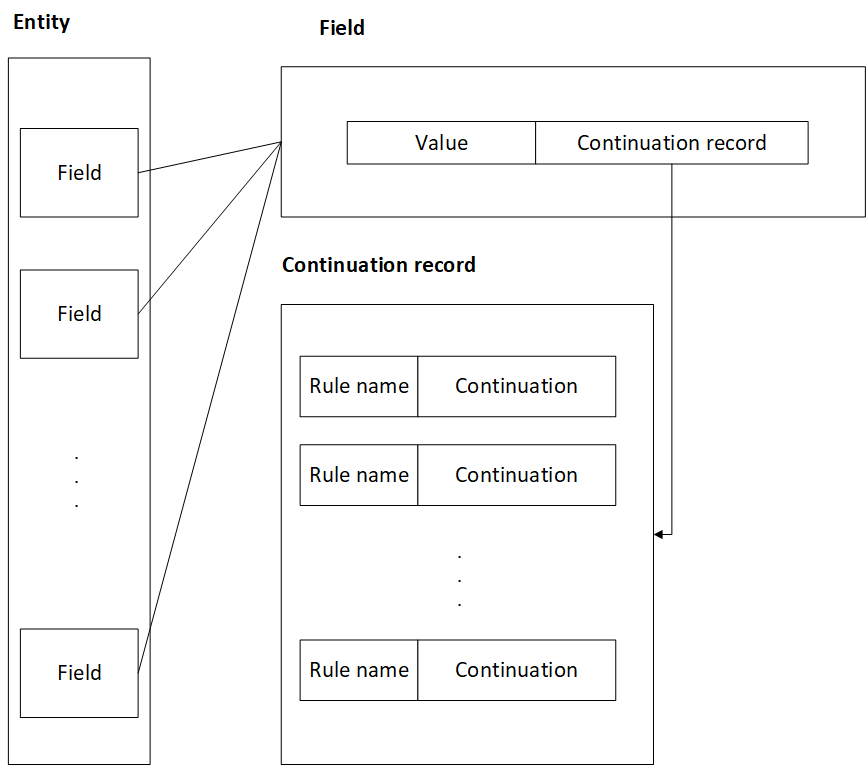
\includegraphics[width=\textwidth]{Figures/chapter_networking/interruptible_rules}
  \caption{Schematic representation of the implementation of the interruptible rules}
  \label{fig:ch_networking_interruptible_rules}
\end{figure}

A field of the entity record must be adapted now to contain not only the field value, but a record instance used to store the continuations of the Casanova rules affecting that field. Since a record requires a name for each field, we can expand the coroutine functor to take a string representing an identifier for each rule and the continuation record itself:

\begin{lstlisting}
Functor "Coroutine" => string => Record => Record => string => stmt : FieldUpdater


---------------------------
Coroutine ruleId continuation r name => FieldUpdater r name {
  ...
}
\end{lstlisting}

\noindent
Now the first string in the declaration of the functor represents the rule identifier, while the other arguments have the same semantics (record and field of the record the rule can modify). When a Casanova statement requires to store the continuation it can use \texttt{ruleId} to build the setter for the record field of the continuation record. It then calls the function \texttt{set} from the setter module instance to save the continuation of each rule. In this way every rule acting on the record is able to store separately its continuation in the continuation record. As an example, we provide below the evaluation rule for the \texttt{wait} statement that updates the continuation in this implementation:

\begin{lstlisting}
t > 0.0
GetField r name => getter
getter.get entity -> (v,cont)
SetField cont ruleId => continuationSetter
continuationSetter.set (wait(t - dt);k) -> cont'
---------------------------------------------
eval_s entity (wait t;k) dt => (v,cont')
\end{lstlisting}

\noindent
Another aspect that has not been considered yet is how to define variables local to the rule (local bindings). Since the set of local bindings is known at compile time, we can modify the continuation record to store not only the continuation itself, but also the state of the local bindings as record of bindings. In this way an element of the continuation record, that we can now call rule state, stores not only the statements of the rule left to evaluate but also the state of the local bindings. When we need to read the value of a binding or update it, we can again use a getter or setter by accessing the rule state and getting or setting the appropriate field for the binding from the binding record. A schematic representation of this implementation can be seen in Figure \ref{fig:ch_networking_interruptible_rules_with_state}.

\begin{figure}
  \centering
  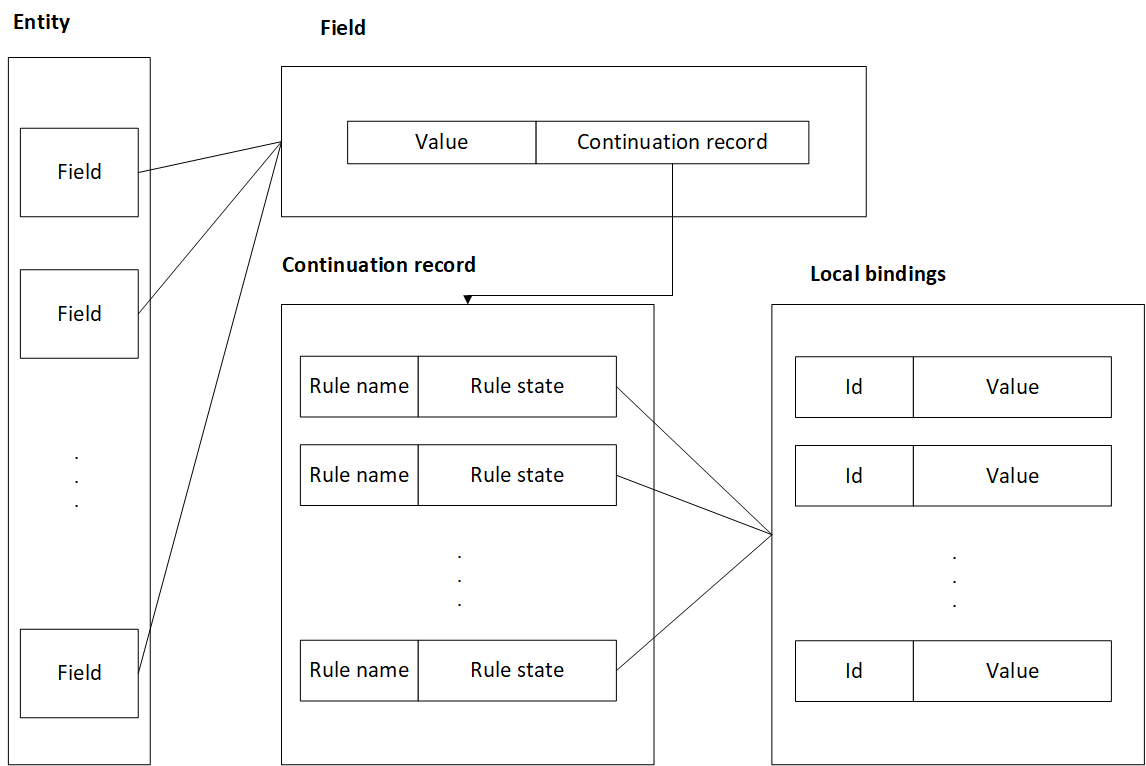
\includegraphics[width=\textwidth]{Figures/chapter_networking/interruptible_rules_with_state}
  \caption{Schematic representation of the implementation of interruptible rules with local bindings}
  \label{fig:ch_networking_interruptible_rules_with_state}
\end{figure}

As final remark, we point out that the use of records to store the rule continuations and local bindings show how the record optimization introduced in Chapter \ref{ch:functors} can also be adapted to implement a generic symbol table to store various information regarding the language elements that are needed during the execution of the generated code, thus making this approach extremely flexible for different situations.

\section{Evaluation}
\label{subsec:ch_functor_languages_evaluation}
In the previous sections we showed how to use functors to implement the entity update traversal of the domain-specific language for game development Casanova. Based on the preliminary analysis performed in Chapter \ref{ch:functors}, we claimed that using functors would improve the performance of the implementation of Casanova in Metacasanova given in Chapter \ref{ch:languages} by, at the same time, inlining the access to the entity fields and pre-building the traversal for the Casanova program at compile time, instead of dynamically accessing the fields from a dictionary and inspecting their type to perform the update traversal at every update. In this section we show the experimental results that show the performance of this implementation in comparison to the first dynamic implementation presented in Chapter \ref{ch:languages}.

\subsection{Experimental Setup}
For this evaluation we have implemented the physical body simulation that was presented in the previous sections. The simulation has been run for 10000 frames, which roughly correspond to 3 minutes assuming an average update rate of 60 frames/second, with a number of physical bodies ranging from 100 to 1000. Each physical body is randomly generated, that is, its initial position, velocity, and acceleration is randomly generated. We measured the time at the beginning and at the end of the execution of the whole simulation and we averaged the total time by the number of frames the simulation has been running for. We then compared the result with what obtained for the implementation shown in Chapter \ref{ch:languages}.

\subsection{Results}
In Table \ref{tab:ch_networking_evaluation} we can see that the update time is in the order of milliseconds or one tenth of milliseconds where the dynamic implementation was in the order of one hundredth of seconds with 1000 entities. This corresponds roughly to a frame rate of 939 frames/second for the functor implementation versus 28 frames/second. The performance gain ranges from a maximum of 55.397 to a minimum of 33.117 times with an avarage gain of 42.508 times. This comes at no surprise, since in Section \ref{sec:ch_functors_evaluation} we tested the gain of accessing record fields with the functor implementation compared to the dynamic tables, and we had an average gain of roughly 11 times. The gap with the dynamic implementation here is even greater because, to the cost of accessing dynamic tables at runtime to retrieve the values of the entity fields, we have to add the performance loss of performing the update traversal and the rule execution dynamically. Figure \ref{fig:ch_networking_chart} shows a chart where the horizontal axis represents the number of entities in the simulation, while the horizontal axis represents the average frame update time with that number of entities in seconds.

To conclude, we want to point out that this evaluation is a worst-case scenario, since the implementation shown in this Chapter makes use exclusively of Metacasanova meta-data structures to represent the values of the entity fields while the simulation shown in Chapter \ref{ch:languages} uses \texttt{Vector2} from the Monogame library. This means that this simulation has an additional overhead due to accessing the components of a tuple via pattern matching, and due to the use of value types versus reference types. The performance shown here could be improved by using \texttt{Vector2} from an external library instead of \texttt{Tuple[float, float]} to store the position, velocity, and acceleration of a physical body.
\begin{table}
  \resizebox{\textwidth}{!}{
  \begin{tabular}{|c|c|c|}
  \hline
  \textbf{Language implementation} & \textbf{Entity number} &	\textbf{Update time}\\
  \hline
  \multirow{5}{*}{Functors}
  & 100 &	0.000063\\
  & 250 &	0.000173\\
  & 500 &	0.000428\\
  & 750 &	0.000777\\
  & 1000 & 0.001065\\
  \hline
  \multirow{5}{*}{Dynamic}
  & 100 & 0.00349\\
  & 250 & 0.00911\\
  & 500 & 0.01716\\
  & 750 & 0.02597\\
  & 1000 & 0.03527\\
  \hline
  \end{tabular}}\\
  
  \vspace{0.5cm}
  \begin{tabular}{|c|c|}
  \hline
  \textbf{Entity number} & \textbf{Performance Gain}\\
  \hline
  100 &	55.397\\
  250 &	52.659\\
  500 &	40.093\\
  750 &	33.423\\
  1000 & 33.117\\
  \hline
  \textbf{Average gain} & 42.938 \\
  \hline
  \end{tabular}
 	\caption{Update time for one frame of the functor implementation of Casanova and the dynamic implementation shown in Chapter \ref{ch:languages}. The time is measured in seconds}
  \label{tab:ch_networking_evaluation}
\end{table}

\begin{figure}[!h]
  \centering
  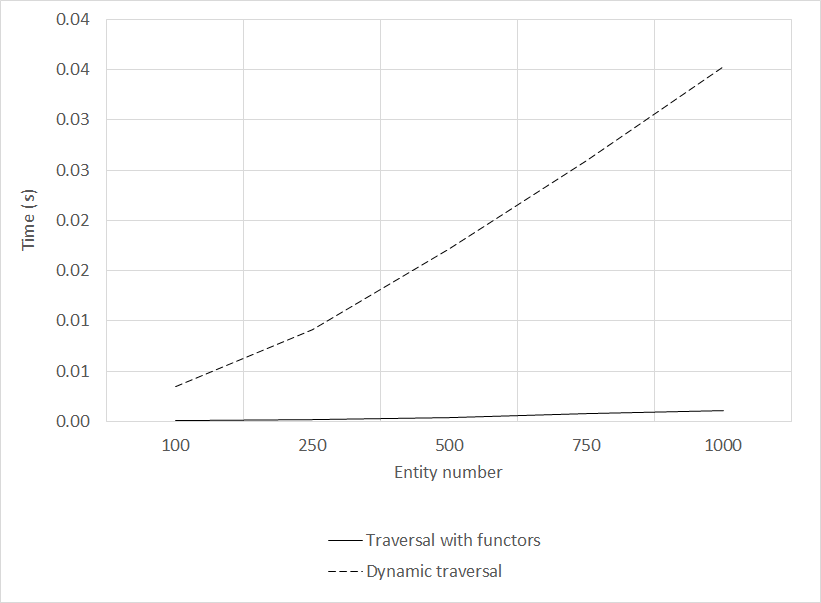
\includegraphics[width=\textwidth]{Figures/chapter_networking/chart}
  \caption{Execution time of Casanova implemented with functors vs the dynamic implementation}
  \label{fig:ch_networking_chart}
\end{figure}

\section{Summary}
In this chapter we proposed a new implementation of the semantics of Casanova based on the language extension with functors and modules presented in Chapter \ref{ch:functors}. We showed that functors and modules are expressive enough to implement the logic of the entity update in Casanova and at the same time to allow rule interruption. At the same time, functors grant static typing and the inlining of ad-hoc update functions depending on the structure of the entity we need to update. This improvement increases the performance of this new implementation of Casanova on average by roughly 42 times. This improvement makes the implementation of Casanova suitable for game development, as the generated code is now able to process at more than 900 frames/second versus the 28 of the previous implementation.
